The model for time evolution of the temperature field~$T$ is thermal diffusion,
which in a plasma gives
\begin{equation}\label{eq:plas2diff}
\frac{3}{2} N \frac{\partial T}{\partial t}=\nabla \cdot \mathcal{K}  \nabla T
\end{equation}
where the thermal conductivity tensor is $\mathcal{K}$.
(Compare the model for a solid
\begin{equation}\label{eq:solidiff}
\rho_m c_p \frac{\partial T}{\partial t}=\nabla \cdot k_c \nabla T
\end{equation}
where the thermal conductivity tensor is $k_c$, $\rho_m$ is the mass density of the medium 
and $c_p$ is its specific heat at constant pressure, implying
that the thermal diffusivity tensor is $\kappa=k_c/\rho_m c_p$.)
Introducing vector components as  in \Sec{intro},
thermal diffusion in a plasma after Braginskii is thus
\begin{equation}\label{eq:plas2brag}
\frac{3}{2} N \frac{\partial T}{\partial t}=
\nabla \cdot \left(
\mathcal{K}_{\|} {\bf b} [{\bf b}.\nabla T] +
\mathcal{K}_{\perp} (\nabla T - {\bf b} [{\bf b}.\nabla T])+
\mathcal{K}_{\wedge} {\bf b} \times \nabla T
\right) 
\end{equation}

Henceforth, the `wedge' transport ie. in due to the term in $\mathcal{K}_{\wedge}$
is neglected for the reason that it may be rearranged to give
a convection-like term, via the identity 
\begin{equation}\label{eq:crossxp}
\nabla \cdot \mathcal{K}_\wedge {\bf b} \times \nabla T = \nabla \cdot ({\bf u}_\wedge  T)
\end{equation}
where
\begin{equation}\label{eq:uxp}
{\bf u}_\wedge = \nabla \times (\mathcal{K}_\wedge {\bf b})
\end{equation}
(In any event, if $\mathcal{K}_\wedge$ is a function purely of~$T$, and
$\nabla \cdot {\bf b}=\bf{0}$, then the terms in \Eq{crossxp} vanish.)

Expressions for the thermal diffusivities $\kappa_{\perp}$ and~$\kappa_{\|}$ for
the different species
are given in \Sec{coefficient}, where they incorporate  the factor $\frac{3}{2} N$,
ie.\ $\kappa_{(\perp , \|) e,i}=\mathcal{K}_{(\perp, \|)}/(\frac{3}{2} N)$.

\subsection{Test Cases}\label{sec:tests}
The aim of the work is to calculate in a series of calculations that increasingly
approach the realistic model, the magnitude of the spurious numerical diffusion
perpendicular to the magnetic field direction~${\bf b}$. The main interest concerns
how much diffuses in the plasma, not the solid surface, even though the deposition
of power is on the surface, reason: all sorts of complicated extra physics come
into play in the plasma especially near surfaces.
\subsubsection{Starting Case}\label{sec:start}
For the 2-D test case illustrated in \Fig{aniso}, it is suggested that $\kappa_{\perp}=0$
so that any perpendicular diffusion is numerical in origin. Given this,
the problem can be analysed using any spatial scale and any convenient~$\kappa_{\|}$.
However an order of magnitude estimate for tile dimensions is one metre,
discharge timescale is one second upwards. For plasma properties
assume $N=10^{18}$\,m$^{-3}$, $T_i=T_e=10$\,eV, $Z=A=1$, $B=3$\,T and solid temperatures say $500^o$\,C.

In \Fig{aniso}, $T=T_0>0$ over the interval on the left hand boundary that is connected by field
in direction~${\bf b}$ with the thick red line,
elsewhere on the blue fieldlines, $T=0$. The red region lies on a black line
which denotes the boundary between anisotropic conductor and  perfect insulator. 
The exact steady-state solution has $T=constant$ along fieldlines, but numerical
diffusion will result in non-zero~$T$ in the region of blue fieldlines.
The relative size of this numerical diffusion must be estimated as a function
of incidence angle~$\theta$, where interest attaches to small $\theta\leq2^o$.
\begin{figure}
\centerline{
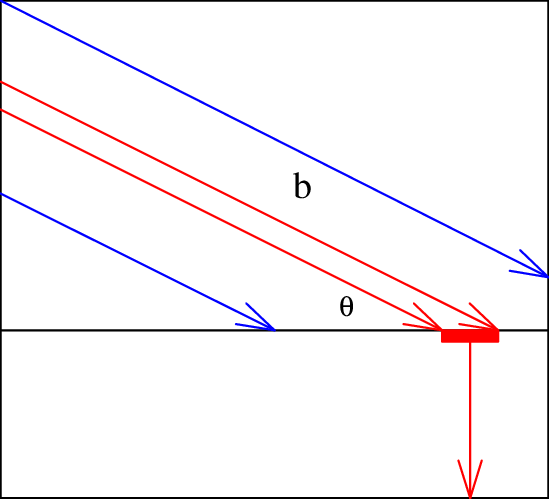
\includegraphics[width=8.0cm]{../png/aniso.png}
}
\caption{Sketch of the test configuration, showing fieldlines in direction~${\bf b}$
and the boundary between anisotropic conductor and perfect insulator.
\label{fig:aniso}}
\end{figure}

\subsubsection{Intermediate Case}\label{sec:intermediate}
To test curvature effects the whole 2-D domain of \Fig{aniso} could be distorted by conformal mapping
(which preserves angles).

\subsubsection{Realistic Case}\label{sec:realistic}
This needs to be 3-D and involve JET divertor tile descriptions derived from
the output of the CAD design tool, together with information
describing the magnetic field as a function of position, which will be supplied.
The magnetic equilibrium may be supplied analytically after Solovev, but the
usual input is as an .eqdsk file.
The EQDSK~G format is a ``non-standard" standard for
solutions $\psi(R,Z), p(\psi), I(\psi)$ of the Grad-Shafranov equation, where
$\psi$ is the magnetic flux and $(R,Z)$ are cylindrical coordinates
in planes normal to the toroidal direction. The functions~$p$ and~$I$ give the
variation of the pressure and toroidal field respectively.
The basic standard for EQDSK~G may be found at:
\url{https://fusion.gat.com/theory/Efitgeqdsk} (which may be password-protected)
or else at ~\url{https://w3.pppl.gov/ntcc/TORAY/G_EQDSK.pdf}
The flux~$\psi(R,Z)$ is sampled at uniformly spaced points on a direct product grid,
for which the .eqdsk header defines the mesh-size, as well as other useful
information, such as the flux on axis and at boundary.
Unfortunately the strict EQDSK~G standard uses a Fortran format that does
not require spaces between samples, hence there are many variants for
languages that cannot handle this situation, that have introduced other
features such as mistakes in field helicity, factors of $2\pi$ in the flux, etc.
Routines that calculate magnetic field~${\bf B}$ using cubic spline interpolation
could be made available. It would be desirable for the output of System 2-2
to be used.


\subsubsection{Extended Case}\label{sec:extended}
An extended test would allow for heat transfer in the solid surface sketched 
at bottom of \Fig{aniso}, taking say thermal diffusivity for Tungsten
$\kappa \approx 3 \times 10^{-5}$\,m$^2$ s$^{-1}$. 
%\begin{figure}
%\centerline{
%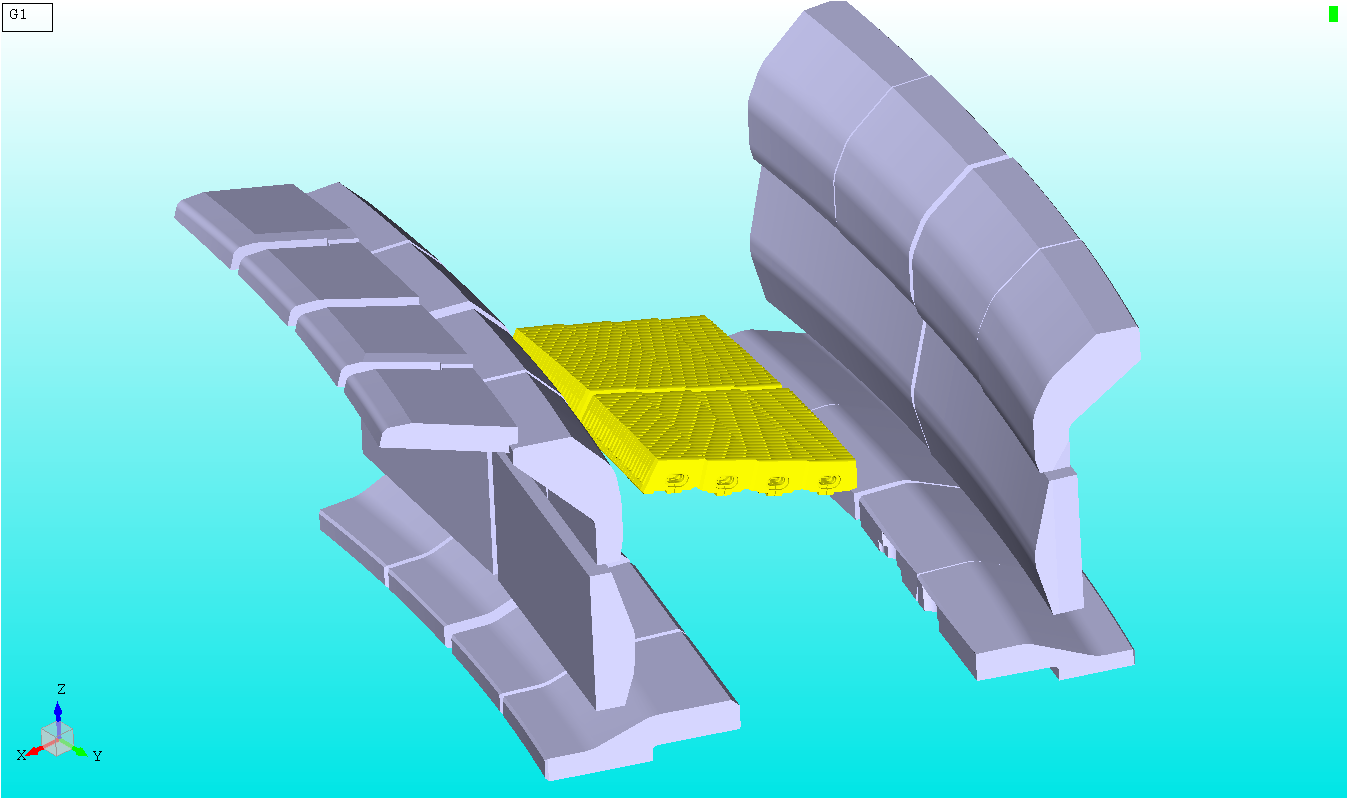
\includegraphics[width=8.0cm]{../png/pretty}
%}
%\caption{CAD for JET divertor after simplification. A $15^o$ sector in toroidal angle is shown,
%except for the T5~armour, where only $7.5^o$ are drawn. The magnetic field (not shown)
%is predominantly directed in the toroidal direction to achieve near grazing incidence.
%\label{fig:pretty}}
%\end{figure}
